%% ---- sezione E: generazione ----
\section{Generazione di scenari sintetici e validazione}

\paragraph{Dal prior al block-bootstrap storico (\S8.1).}
La regolarizzazione di Kullback-Leibler permette in linea di principio di generare nuove matrici decodificando $\mathbf{z} \sim \mathcal{N}(0, I)$ campionato dal prior. L'obiettivo della tesi non è però uno scenario plausibile qualsiasi, bensì una distribuzione di scenari sintetici della struttura di correlazione a orizzonte nominale di 21 giorni lavorativi, costruiti ricampionando transizioni storiche dello spazio latente a partire dallo stato di mercato osservato. Non si tratta di previsioni puntuali, ma di una stima della possibile variabilità delle correlazioni a quell'orizzonte, in ottica di rischiosità. Il campionamento dal prior è perciò sostituito da un block-bootstrap storico nello spazio latente (modello \texttt{VAE\_20dim\_cholesky\_06\_loss}):
\begin{enumerate}
\item l'encoder è applicato all'intera serie storica a passo giornaliero (stride 1): 4124 punti latenti;
\item si calcolano gli incrementi giornalieri $\Delta \mathbf{z}_t = \mathbf{z}_t - \mathbf{z}_{t-1}$;
\item si estrae casualmente un blocco di 21 incrementi consecutivi (un mese lavorativo), sommati in $\delta \mathbf{z}$;
\item il salto si somma allo stato attuale: $\mathbf{z}_{\mathrm{futuro}} = \mathbf{z}_{\mathrm{oggi}} + \delta \mathbf{z}$;
\item il decoder produce il fattore di Cholesky $L$, da cui $C = L L^{\top}$, poi rinormalizzata a diagonale unitaria: la semidefinita positività è garantita per costruzione.
\end{enumerate}
La procedura è ripetuta 1000 volte a partire da $\mathbf{z}_{\mathrm{oggi}}$, che codifica l'ultima matrice reale del dataset (finestra dal 28 febbraio 2018 al 12 gennaio 2021): la ``data odierna'' del capitolo è dunque il 12 gennaio 2021, ultima quotazione disponibile, non la data di stesura. Nella Figura~\ref{fig:scenari} la traiettoria storica esplora un'ampia porzione dello spazio latente, mentre la nuvola dei 1000 scenari resta concentrata in un intorno relativamente ristretto dello stato attuale: la variabilità cumulata su 21 giorni è necessariamente più contenuta di quella del ventennio.

\begin{figure}[htbp]
\centering
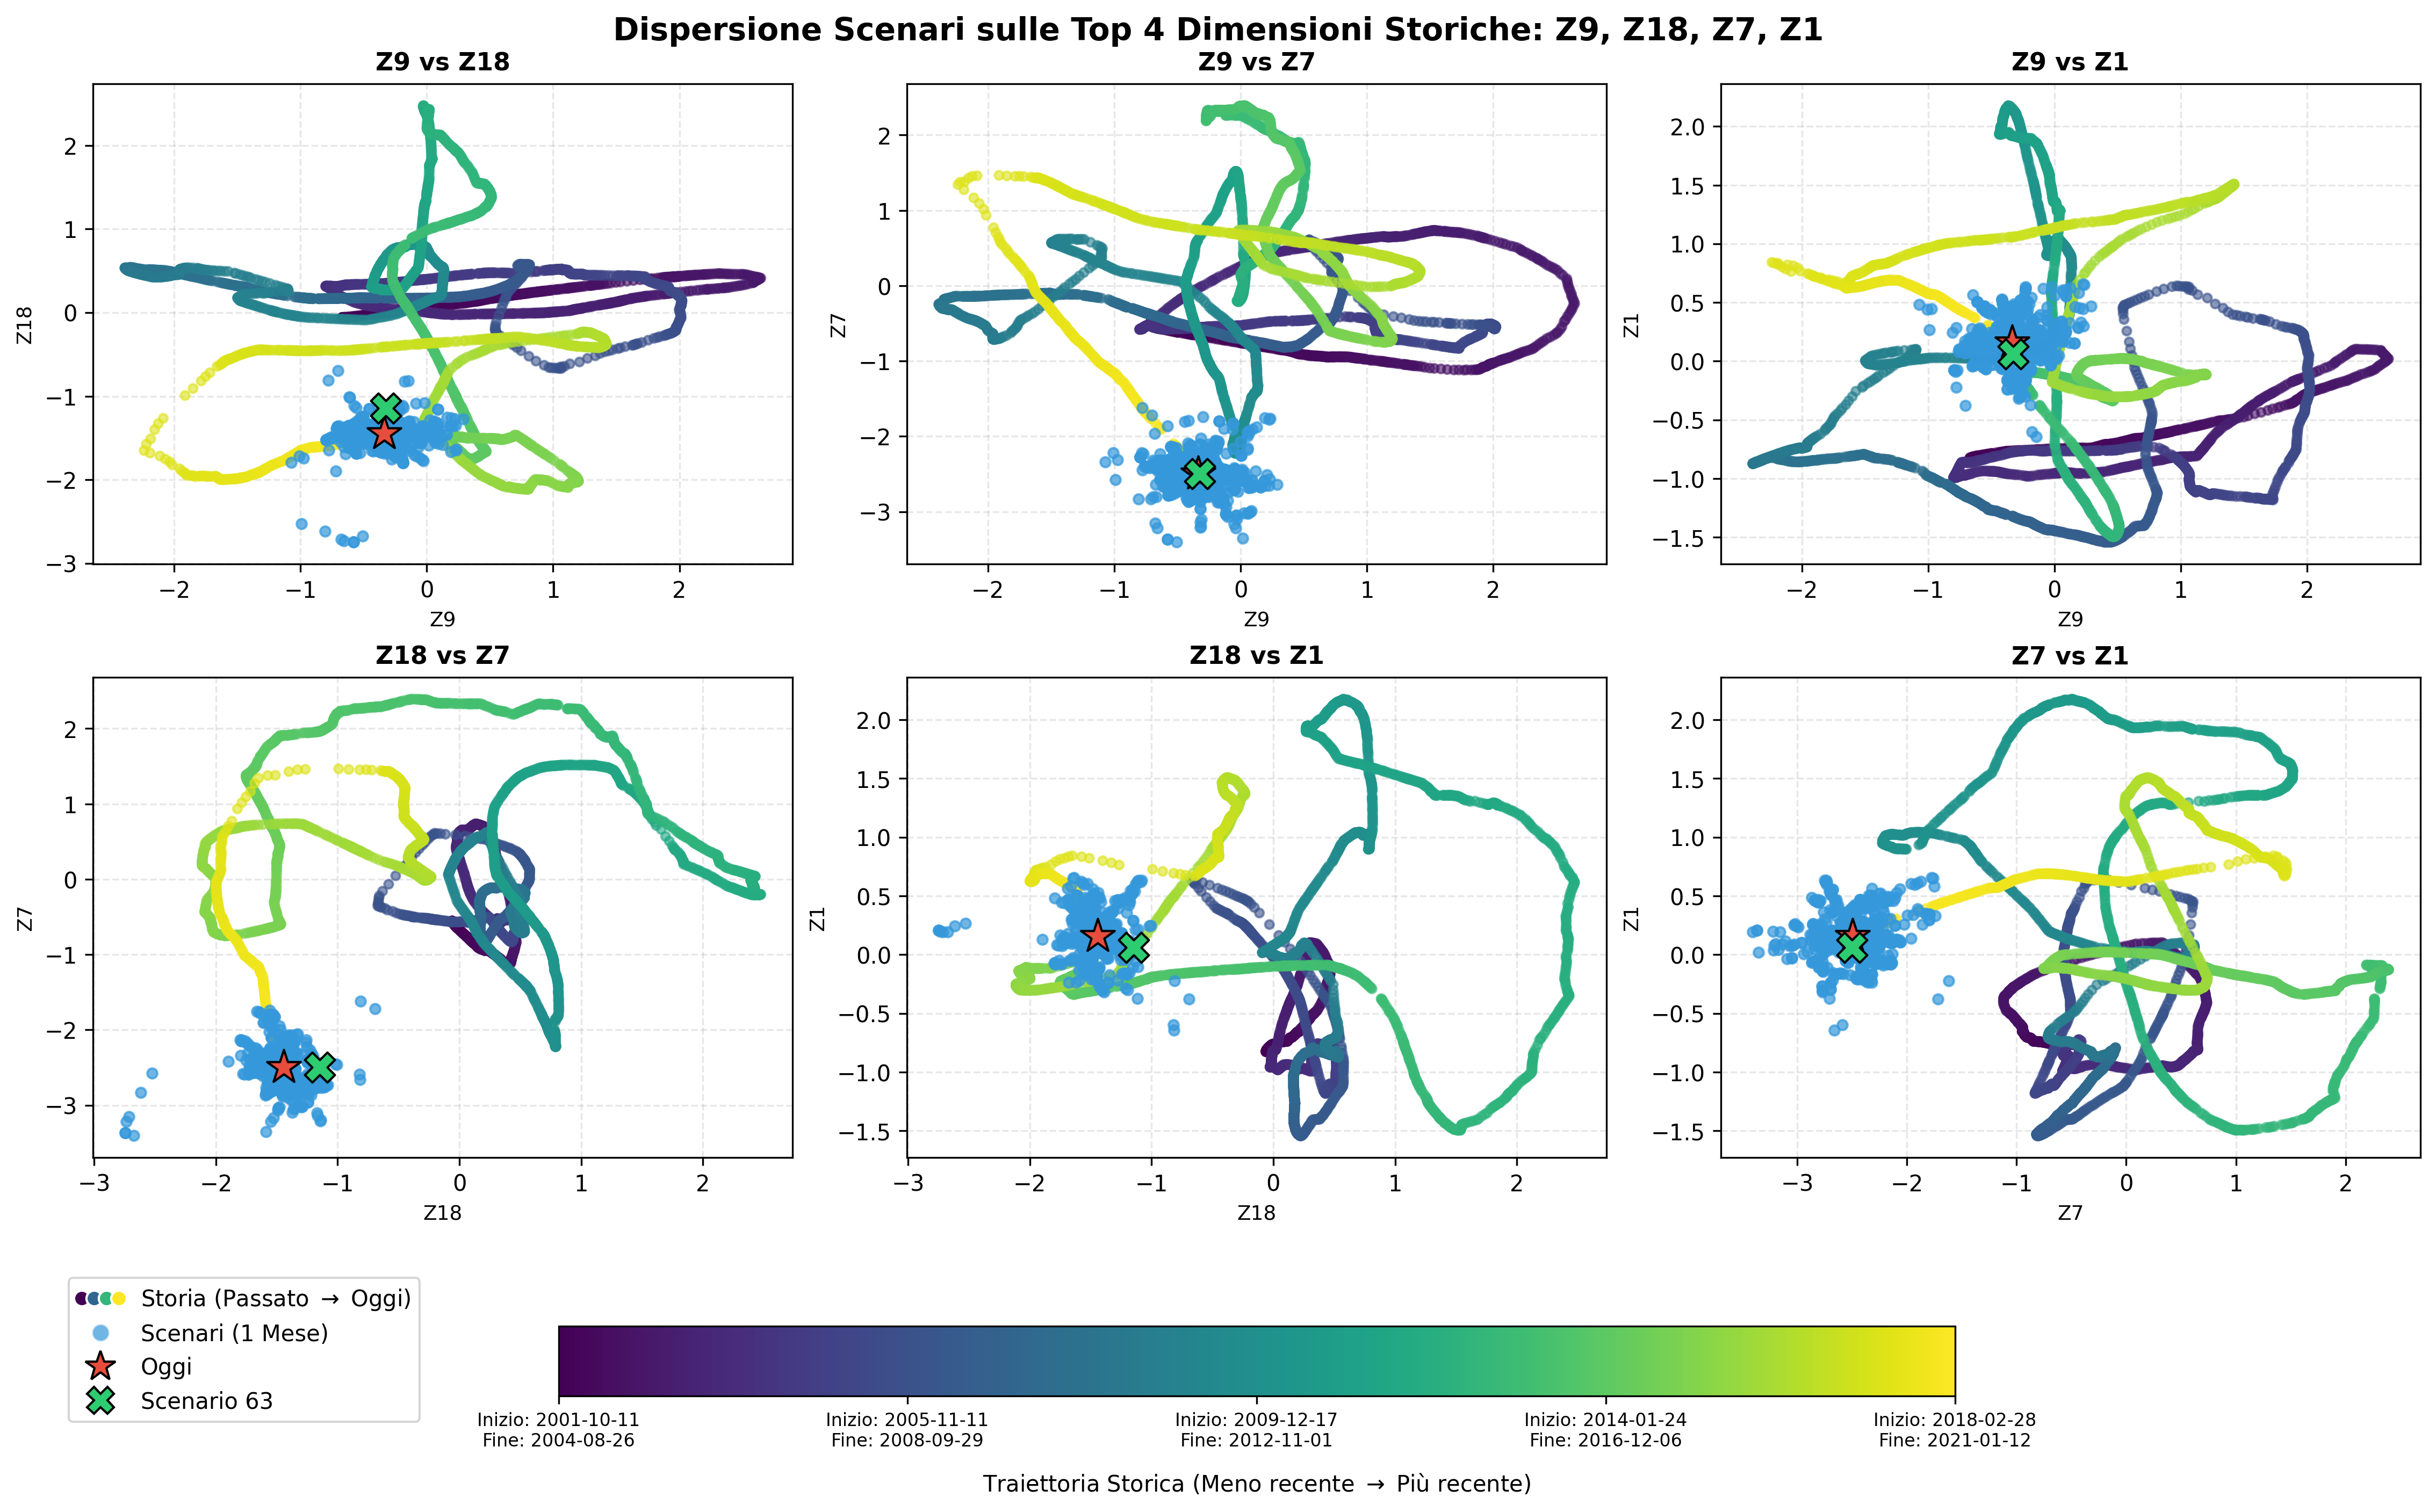
\includegraphics[width=0.9\linewidth]{Pictures/capitolo8/fig_latent_scenarios_scatter_2d.png}
\caption{Proiezioni a coppie sulle quattro dimensioni latenti a maggiore varianza storica ($Z_9$, $Z_{18}$, $Z_7$, $Z_1$): traiettoria storica dalle prime finestre valide (ottobre 2001) all'ultima (gennaio 2021), colore proporzionale al tempo, nuvola dei 1000 scenari a 21 giorni (punti azzurri), stato odierno (stella) e scenario 63 (croce).}
\label{fig:scenari}
\end{figure}

\paragraph{Verifica aggregata sui 1000 scenari (\S8.2.1).}
Ogni scenario è confrontato con la matrice odierna sui cinque fatti stilizzati del cap.~3, tradotti in indicatori scalari: la media dei coefficienti fuori diagonale; l'autovalore di mercato $\lambda_1$ e il numero di autovalori oltre il limite $\lambda_+ = 2.914$ del bulk di Marchenko-Pastur; la componente minima $\min_i v_{1,i}$ del market mode (normalizzato a somma positiva), la cui positività equivale alla proprietà di Perron-Frobenius; il rapporto $R$ fra correlazione media intra-settore e inter-settore GICS, pari a 1 in assenza di struttura settoriale (1.278 sulla matrice odierna); l'esponente $\gamma$ della distribuzione di grado dell'MST. La Tabella~\ref{tab:fatti} riporta i criteri di conformità e i due riferimenti: la matrice odierna e l'intervallo osservato sulle 412 matrici reali del bacino epurato, adottato dove la letteratura non fissa soglie assolute.

Tutti i 1000 scenari soddisfano simultaneamente i cinque fatti; tutte le matrici risultano inoltre definite positive (autovalore minimo fra 0.0101 e 0.0185), in linea con la semidefinita positività garantita per costruzione. I 65.3 milioni di coefficienti aggregati hanno media 0.4628 contro 0.4512 della matrice odierna; $\lambda_1$ resta circa due ordini di grandezza oltre $\lambda_+$; $\gamma$ cade sempre in $(2, 3)$, mentre solo il 64.1\% delle 412 matrici reali vi ricade. La tesi ne propone una spiegazione topologica plausibile: nelle finestre storiche con un hub dominante il grado massimo dell'MST arriva a 36 e la pendenza log-log si appiattisce, mentre negli scenari il grado massimo resta fra 12 e 18.

\begin{table}[htbp]
\centering
\small
\begin{tabular}{@{}llcccc@{}}
\toprule
Fatto stilizzato & Criterio & Scenari (1000) & Odierna & Reali (412) & Conformi \\
\midrule
FS1 Distribuzione & spostamento & [0.4609, 0.5352] & 0.4512 & [0.2240, 0.5070] & 1000/1000 \\
\quad (media pairwise) & \quad positivo & & & & \\
\addlinespace
FS2 Marchenko-Pastur & $\lambda_1 \gg \lambda_+$ & [172.4, 197.2] & 169.1 & [85.4, 186.8] & 1000/1000 \\
\quad ($\lambda_1$; modi $> \lambda_+$) & \quad almeno 2 modi & [7, 9] & 9 & [7, 12] & \\
\addlinespace
FS3 Perron-Frobenius & $> 0$ & [0.0164, 0.0227] & 0.0151 & [0.0007, 0.0288] & 1000/1000 \\
\quad ($\min_i v_{1,i}$) & & & & & \\
\addlinespace
FS4 Gerarchia & $> 1$ & [1.198, 1.268] & 1.278 & [1.165, 1.814] & 1000/1000 \\
\quad ($R$ intra/inter) & & & & & \\
\addlinespace
FS5 MST scale-free & $2 < \gamma < 3$ & [2.053, 2.306] & 2.119 & [1.676, 2.340] & 1000/1000 \\
\quad (esponente $\gamma$) & & & & & \\
\midrule
\multicolumn{5}{@{}l}{Tutti e cinque i fatti stilizzati simultaneamente} & 1000/1000 \\
\bottomrule
\end{tabular}
\caption{Verifica aggregata dei cinque fatti stilizzati sui 1000 scenari generati dal modello \texttt{VAE\_20dim\_cholesky\_06\_loss} (Tabella 8.1 della tesi): intervallo [min, max] sugli scenari, valore della matrice odierna (finestra chiusa il 12 gennaio 2021) e intervallo [min, max] sulle 412 matrici reali del bacino epurato.}
\label{tab:fatti}
\end{table}

\begin{riquadro}{Osservazione: lo scenario 311}
La correlazione media dello scenario 311 (0.5352) supera lievemente l'estremo superiore dell'intervallo tipico $[0.2, 0.5]$ del cap.~3. Non è una violazione: il fatto stilizzato prescrive uno spostamento sistematico verso valori positivi, che uno scenario più correlato soddisfa a maggior ragione, e l'intervallo descrive la magnitudo dei regimi ordinari, non un limite algebrico. Scenari così sincronizzati, tipici delle fasi di stress, sono in ottica di rischiosità la porzione più interessante della distribuzione.
\end{riquadro}

\paragraph{Ispezione dello scenario 63 (\S8.2.2).}
A complemento degli indicatori scalari, la tesi ripercorre graficamente i cinque fatti sullo scenario 63, scelto a fini espositivi. Media e mediana pairwise valgono 0.4635 e 0.4711 contro 0.4512 e 0.4593 della matrice odierna; $\lambda_1$ vale 173.2 contro 169.1, con nove autovalori oltre il bulk in entrambe. Il market mode ha componenti tutte dello stesso segno e similarità coseno 0.9999 con quello odierno (0.9893 e 0.9883 per il secondo e il terzo autovettore); il dendrogramma ripropone gli stessi blocchi settoriali GICS; l'esponente scale-free è 2.227 contro 2.119, con grado massimo 14 contro 15.
